\title{\textbf{Text Analytics} \\ 1\textsuperscript{st} Assignment}
\author{

        Kyrkos Konstantinos - p3351907\\
        
}
\date{\today}


\documentclass[11pt]{article}

\usepackage{tikz}
\usetikzlibrary{shapes,backgrounds}
\usepackage{fancyhdr}
\usepackage{amsmath}
\usepackage{amssymb}
\usepackage{listings}
\usepackage{hyperref}
%\usepackage{graphicx}
\usepackage{enumitem}
\graphicspath{ {./images/} } 
%\usepackage[showframe]{geometry}
\fancypagestyle{headings}{
\cfoot{\thepage}
}

\begin{document}
\maketitle

This report is one of the two deliverables which we provide as solution for the 1st Assignment for the course of Text Analytics for the MSc in Data Science at Athens University of Economics and Business. 

Below we provide an overview of what we have created, explanations for methods and patterns used, descriptions and opinions on tools, algorithms and practices.

%add colab link

\section*{Exercise 4}

For the purpose of this excercise we have implemented the below parts. In each part we explain all code used for the assignment.

\subsection*{Part i.}
S
In the first section we have to implement a bigram and a trigram language model for word sentences. 
We start by loading all the libraries we will later use in our code and then we download the \textbf{Brown} corpus\footnote{ the Brown corpus was the first million-word electronic corpus of English, created in 1961 at Brown University} using NLTK. After having observed some issues with our corpus, which made it harder to manipulate, we replaced some characters for ease of use. For example we replaced multiple questionmarks or exclamation marks with single ones. 

Next, using the afforementioned corpus we first split it into sentences using a package provided by NLTK. We randomly shuffle \footnote{shuffling the sentences makes the training more unbiased, because in this way we sample sentences uniformly from different topics inside the corpus.} the sentences and assign them into three different sets:
\begin{itemize}
\item
The largest set, will be our training set, consisting of the \textbf{70\%} of the corpus. 
\item The next part, will be the development set, which will be used for parameter tuning and consists of the \textbf{20\%} of the corpus. 
\item The final part, will be our test set consisting of the remaining \textbf{10\%} of our corpus.
\end{itemize}

Futhermore, we move on to create our vocabulary and our tokenized sentences from the training set. In order to do that, we've created a function (\textcolor{red}{\textit{get\_vocabulary}}) that utilizes a word tokenizer using regular expressions and a frequency calculator through NLTK. Of the words we that have found, we only keep those that appear 10 or more times in the training set. 

We have also created another function (\textcolor{red}{\textit{tokenize\_n\_replace}}) which returns tokenized sentences, using the same tokenizer. It also lowercases the words. We chose this uniformity in the cases of the words, because  we believe that it improves the performance of our language models. Lastly, it replaces each word not found in our vocabulary with a special character (\textbf{$<UNK>$}) as suggested by the exercise.

Moving on to the next code block, we used \textbf{\textit{Counter}} from the \textbf{\textit{collections}} package to keep track of n-grams frequencies. This was made possible through python's \textbf{\textit{zip}} function. Worth mentioning here is the addition of the corresponding number of pseudo-tokens (1 for bi-grams and 2 for tri-grams) at the beginning and the end of each sentence (using our \textcolor{red}{\textit{pad}} function), which will later help us calculate the probabilities of the first and last words of each sentence.

In the next three blocks of code provided, we have first implemented two functions for calculating the bi-gram and tri-gram probabilites (\textcolor{red}{\textit{bigram\_prob\_calc}} and \textcolor{red}{\textit{trigram\_prob\_calc}}). For each of these functions, we used the corresponding types for conditional probabilities which are presented below\footnote{For the calculation of the conditional probabilities in each language model, the Markov assumption is being utilized}. 

\begin{align*}
\textbf{Bigram probability: }& P(w_2|w_1) = \frac{C(w_1,w_2)+\alpha}{C(w_1)+\alpha|V|} \\
\textbf{Trigram probability: }& P(w_3|w_1,w_2) = \frac{C(w_1,w_2,w_3)+\alpha}{C(w_1,w_2)+\alpha|V|}
\end{align*}
where 
\begin{itemize}
\item $C(w_1)$: unigram count
\item $C(w_1,w_2)$: bigram count
\item $C(w_1,w_2,w_3)$: trigram count
\item $0 \leq \alpha \leq 1$: smoothing hyper-parameter
\end{itemize}

Thus, an example of the calculated bigram probability $P(\text{had} | \text{they})$:
\begin{verbatim}
bigram_prob_calc('they','had',bigram_counter
      ,unigram_counter,vocabulary,alpha)
Out[36]: 0.06982577424078619
\end{verbatim}

and  an example of the calculated trigram probability $P(\text{own} | \text{by},\text{her})$:
\begin{verbatim}
trigram_prob_calc('by','her','own',trigram_counter
      ,bigram_counter,vocabulary,alpha)
Out[37]: 0.02805358990853914
\end{verbatim}

Next, we also created 2 more functions (\textcolor{red}{\textit{b\_log\_prob}} and \textcolor{red}{\textit{t\_log\_prob}}) in order to calculate the log probabilities of a word sequence using the previous conditional probabilities.

\begin{align*}
&\textbf{Bigram language model: } \\
& log_2(P(w_1^k)) \approx  log_2\left(P(w_1|\textcolor{red}{s}) \times P(w_2|w_1) \times \dots P(w_k|w_{k-1}) \times P(\textcolor{red}{e}|w_k)\right)  \\
= & log_2(P(w_1|\textcolor{red}{s}))+ log_2(P(w_2|w_1))+ \dots + log_2(P(w_k|w_{k-1}))+log_2(P(\textcolor{red}{e}|w_k)) \\
\end{align*}

\begin{align*}
&\textbf{Trigram language model: } \\
& log_2(P(w_1^k)) \approx  log_2\left(P(w_1|\textcolor{red}{s1},\textcolor{red}{s2}) 
\times P(w_2|\textcolor{red}{s2},w_1) 
\times \dots P(\textcolor{red}{e1}|w_{k-1},w_{k}) 
\times P(\textcolor{red}{e2}|w_{k},\textcolor{red}{e1})\right)  \\
= & log_2(P(w_1|\textcolor{red}{s1},\textcolor{red}{s2}) 
+log_2(P(w_2|\textcolor{red}{s2},w_1)) + \dots 
+ log_2(P(\textcolor{red}{e1}|w_{k-1},w_{k}) )
+ log_2(P(\textcolor{red}{e2}|w_{k},\textcolor{red}{e1})) \\
\end{align*}


\newpage
\subsection*{Part ii.}

For this part of the exercise, we have to compare the log-probabilities that our trained models return when given (correct) example sentences from the test subset vs. (incorrect) sentences of the same length (in words) consisting of randomly selected vocabulary words. 
In order to achieve that, we start by creating a new function (\textcolor{red}{get\_random\_sentence}) which returns a sentence consisting of random words from our vocabulary\footnote{The random selection is being made with replacement}. We then, tokenize our test sentences and pick a random one for testing. 
We also produce one random sentence with the same length using our aforementioned function and tokenize it too. 
Utilizing the previously explained functions, we calculate the log-probabilities for both sentences using the two language models and we get the following results:

\begin{verbatim}
Real sentence from test-set: 
i am only a simple soldier .
Random sentence: 
remarkable stem assumptions bore inevitably today uneasy
____________________________________________________________
Bigram log-probabilities:
real sentence:  -50.6208 , random sentence:  -115.2969
Trigram log-probabilities:
real sentence:  -63.5887 , random sentence:  -113.4888
\end{verbatim}

Interpreting the results, it is clear that both models successfully return larger probabilities for real sentences, instead of incorrect ones. We also notice that, the bigram model gives a larger probability to the real sentence than the trigram model does.

In order to remove any hesitation about the comments made above, we repeated the above test 100 times for different sentences in the test set and calculated the difference in log probabilities between the real and the random sentence for both models. 
As we can see in the graph below, we always have a larger difference using the bigram language model. Lastly, in all sentences for both models the real sentences had larger probabilities than the random ones.
\newpage
\begin{figure}[h]
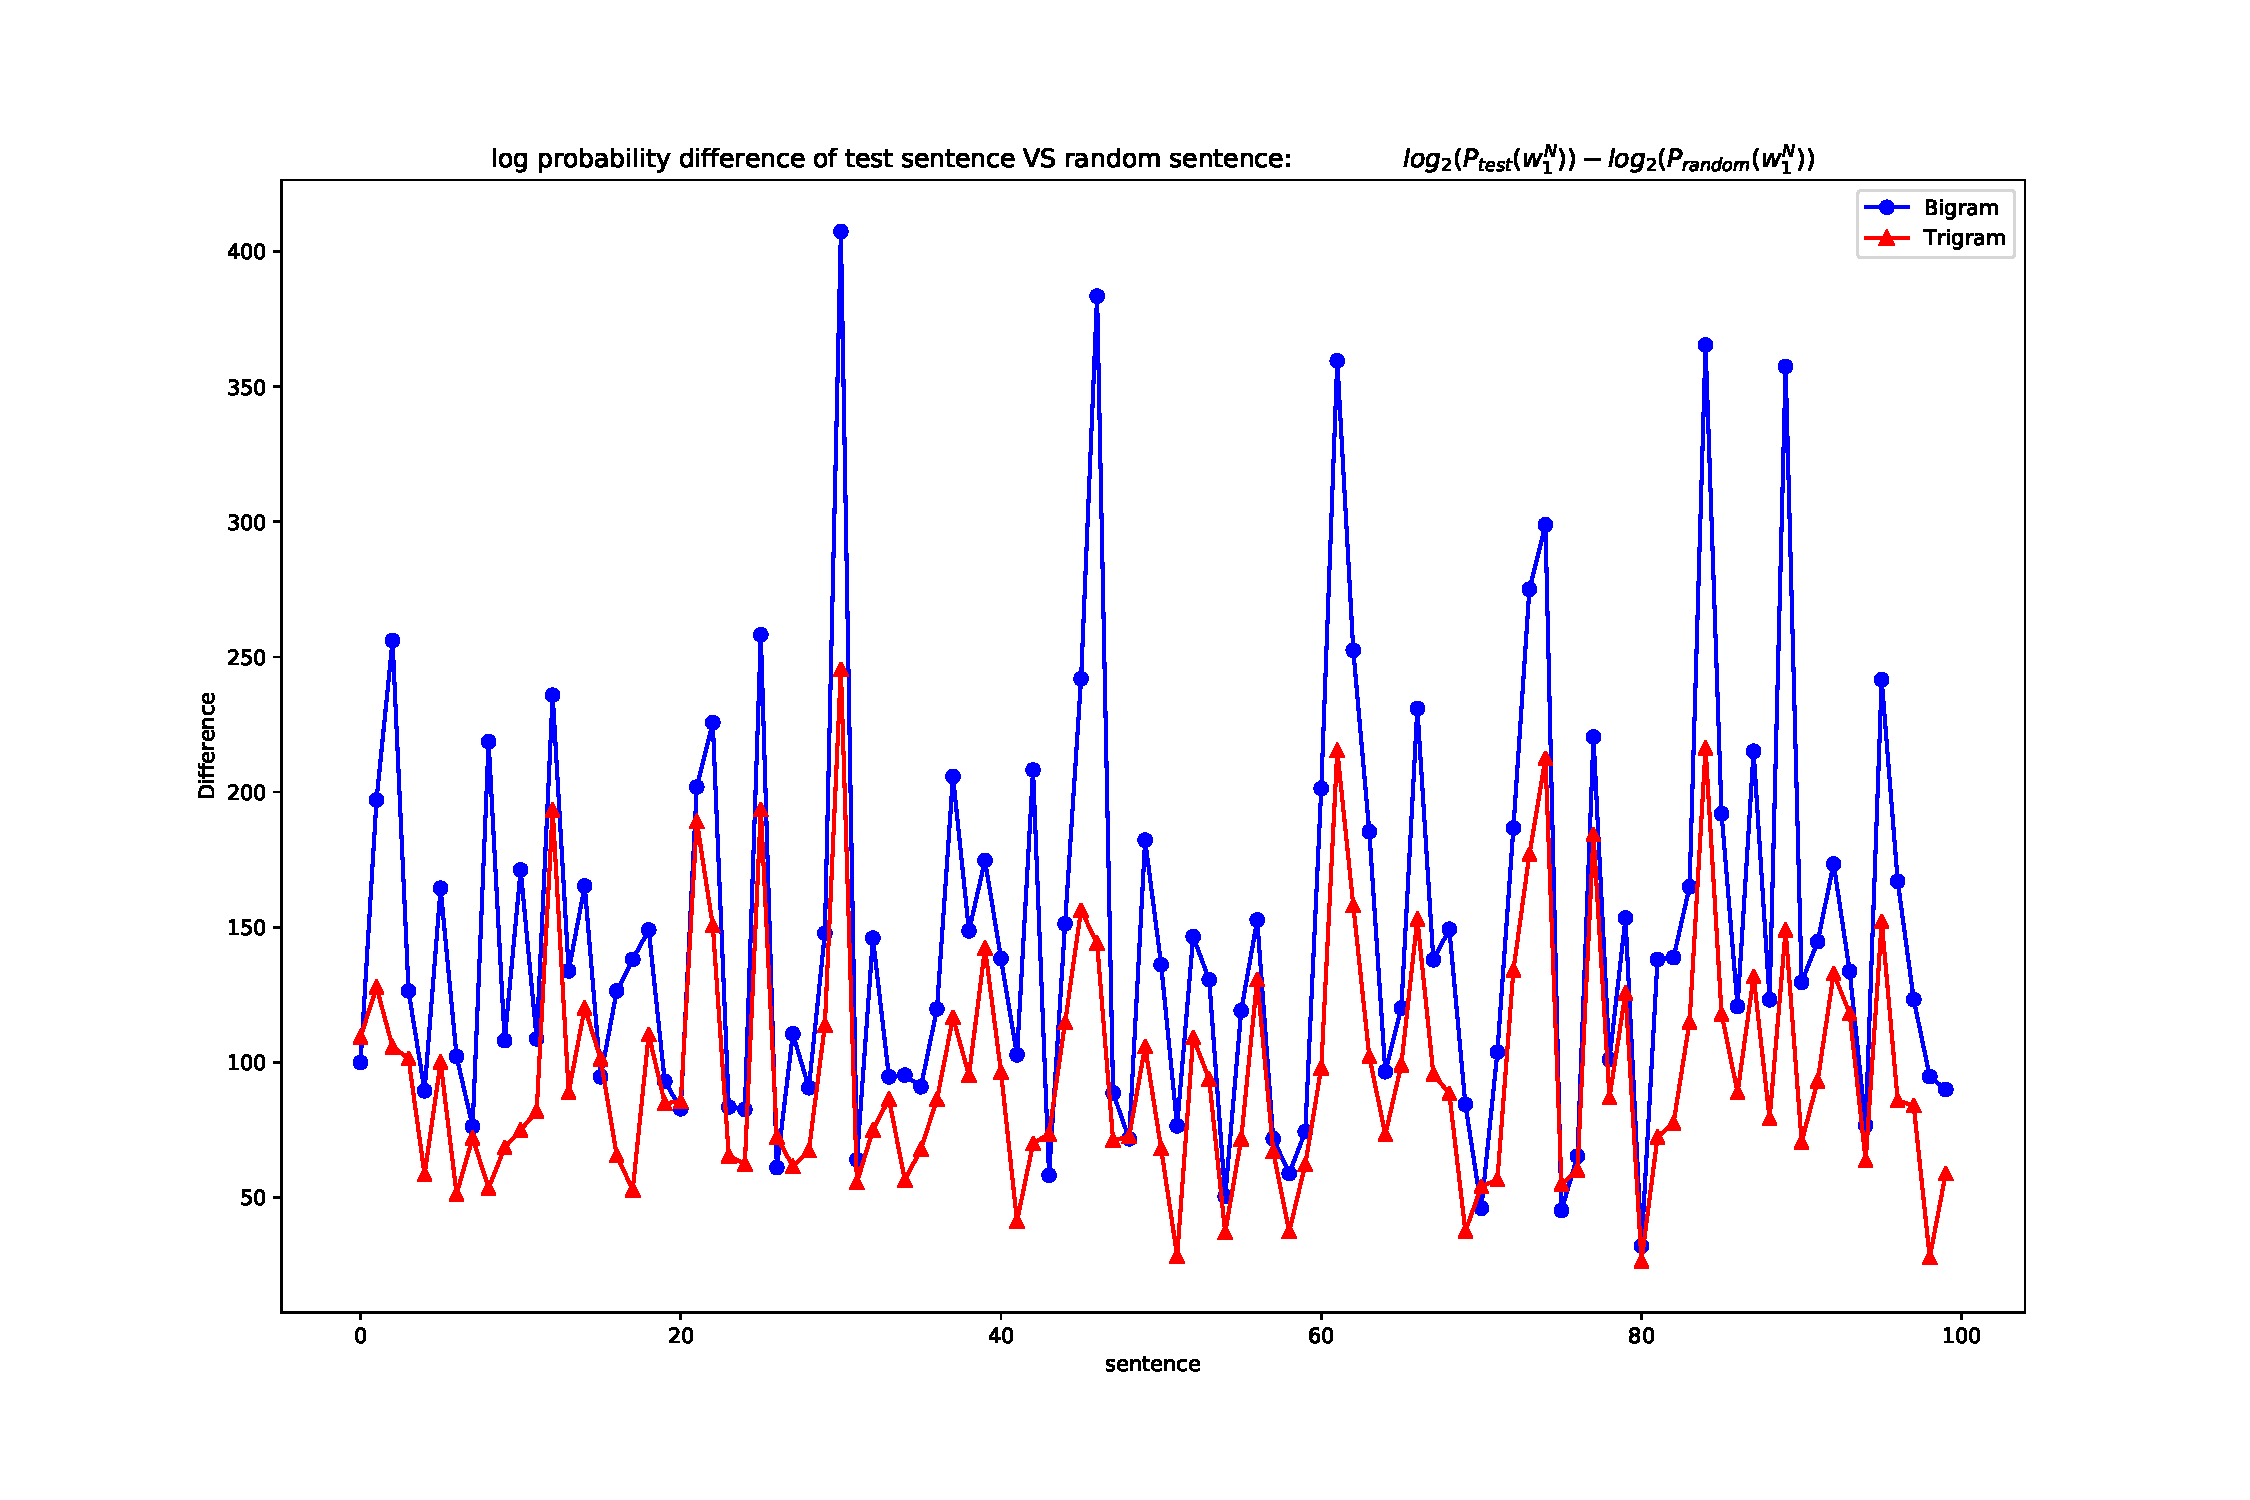
\includegraphics[width=\textwidth]{Real_VS_Random.pdf}
\end{figure}

* We also examined the few sentences where trigrams performed better than bigrams:
\begin{verbatim}
he went to the hotel <UNK> and <UNK> <UNK> .
mr . <UNK> , c . c . b .
we ll work hard , mr . morgan .
no <UNK> for him .
1 and 2 ) .
but not any more .
<UNK> <UNK> .
\end{verbatim}

As we can see, these are very short sentences, consisting of popular phrases ( \textit{not any more, went to the, e.t.c}) and that is why trigrams produced larger differences.

\newpage
\subsection*{Part iii.}
 
For the third part of this exercise, we have to estimate the language cross-entropy and perplexity of our models using a test subset of the corpus, treating the entire test subset as a single sequence. For this purpose, we created a method (\textcolor{red}{CrossEntropy\_Perplexity}) which calculates and returns the values for both cross entropy and perplexity, for a given data set. This method is parameterized to return the values mentioned for the cases of bi-gram, tri-gram and (finally for the purpose of the last part of the assignment) interpolated model.

Moreover, we start by utilizing the above mentioned method to tune the alpha parameter for the add-alpha smoothing. At this point, we make use of the development set we have initially set aside, to be used for parameter tuning, and we tokenize it. Next, we create \textbf{1000} values for the alpha parameter, equally distributed between 0.0001 and 0.5. In these values we are looking to find the optimal hyperparameter, for each of our models. 

Generally, it is known that $H_{P_m}(L)>=H(L)$ where $H(L)$ is the unknown optimal language entropy. We are trying to find a parameter value for $\alpha$ that will lead us to a model with the smallest possible cross-entropy.

\iffalse
The next proccess as described, is initially used for the bi-gram model and after that for the tri-gram model. 

We start the process by calling our method for cross-entropy and perplexity for each of the alphas we have created and gather all the values of perplexity. After this procedure finishes, we  print a graph with all the perplexity values versus their corresponding alpha values in order to have a look at the data we have produced. Next we find the lowest value for perplexity and also its corresponding alpha value and we print these best alpha values for each model. These values are \textbf{0.008} for the bi-gram model and \textbf{0.002} for the tri-gram model. From now on, these values will be used when using add-alpha smoothing as they achieve the best results for the perplexity of the models.
\fi

\begin{figure}[h]
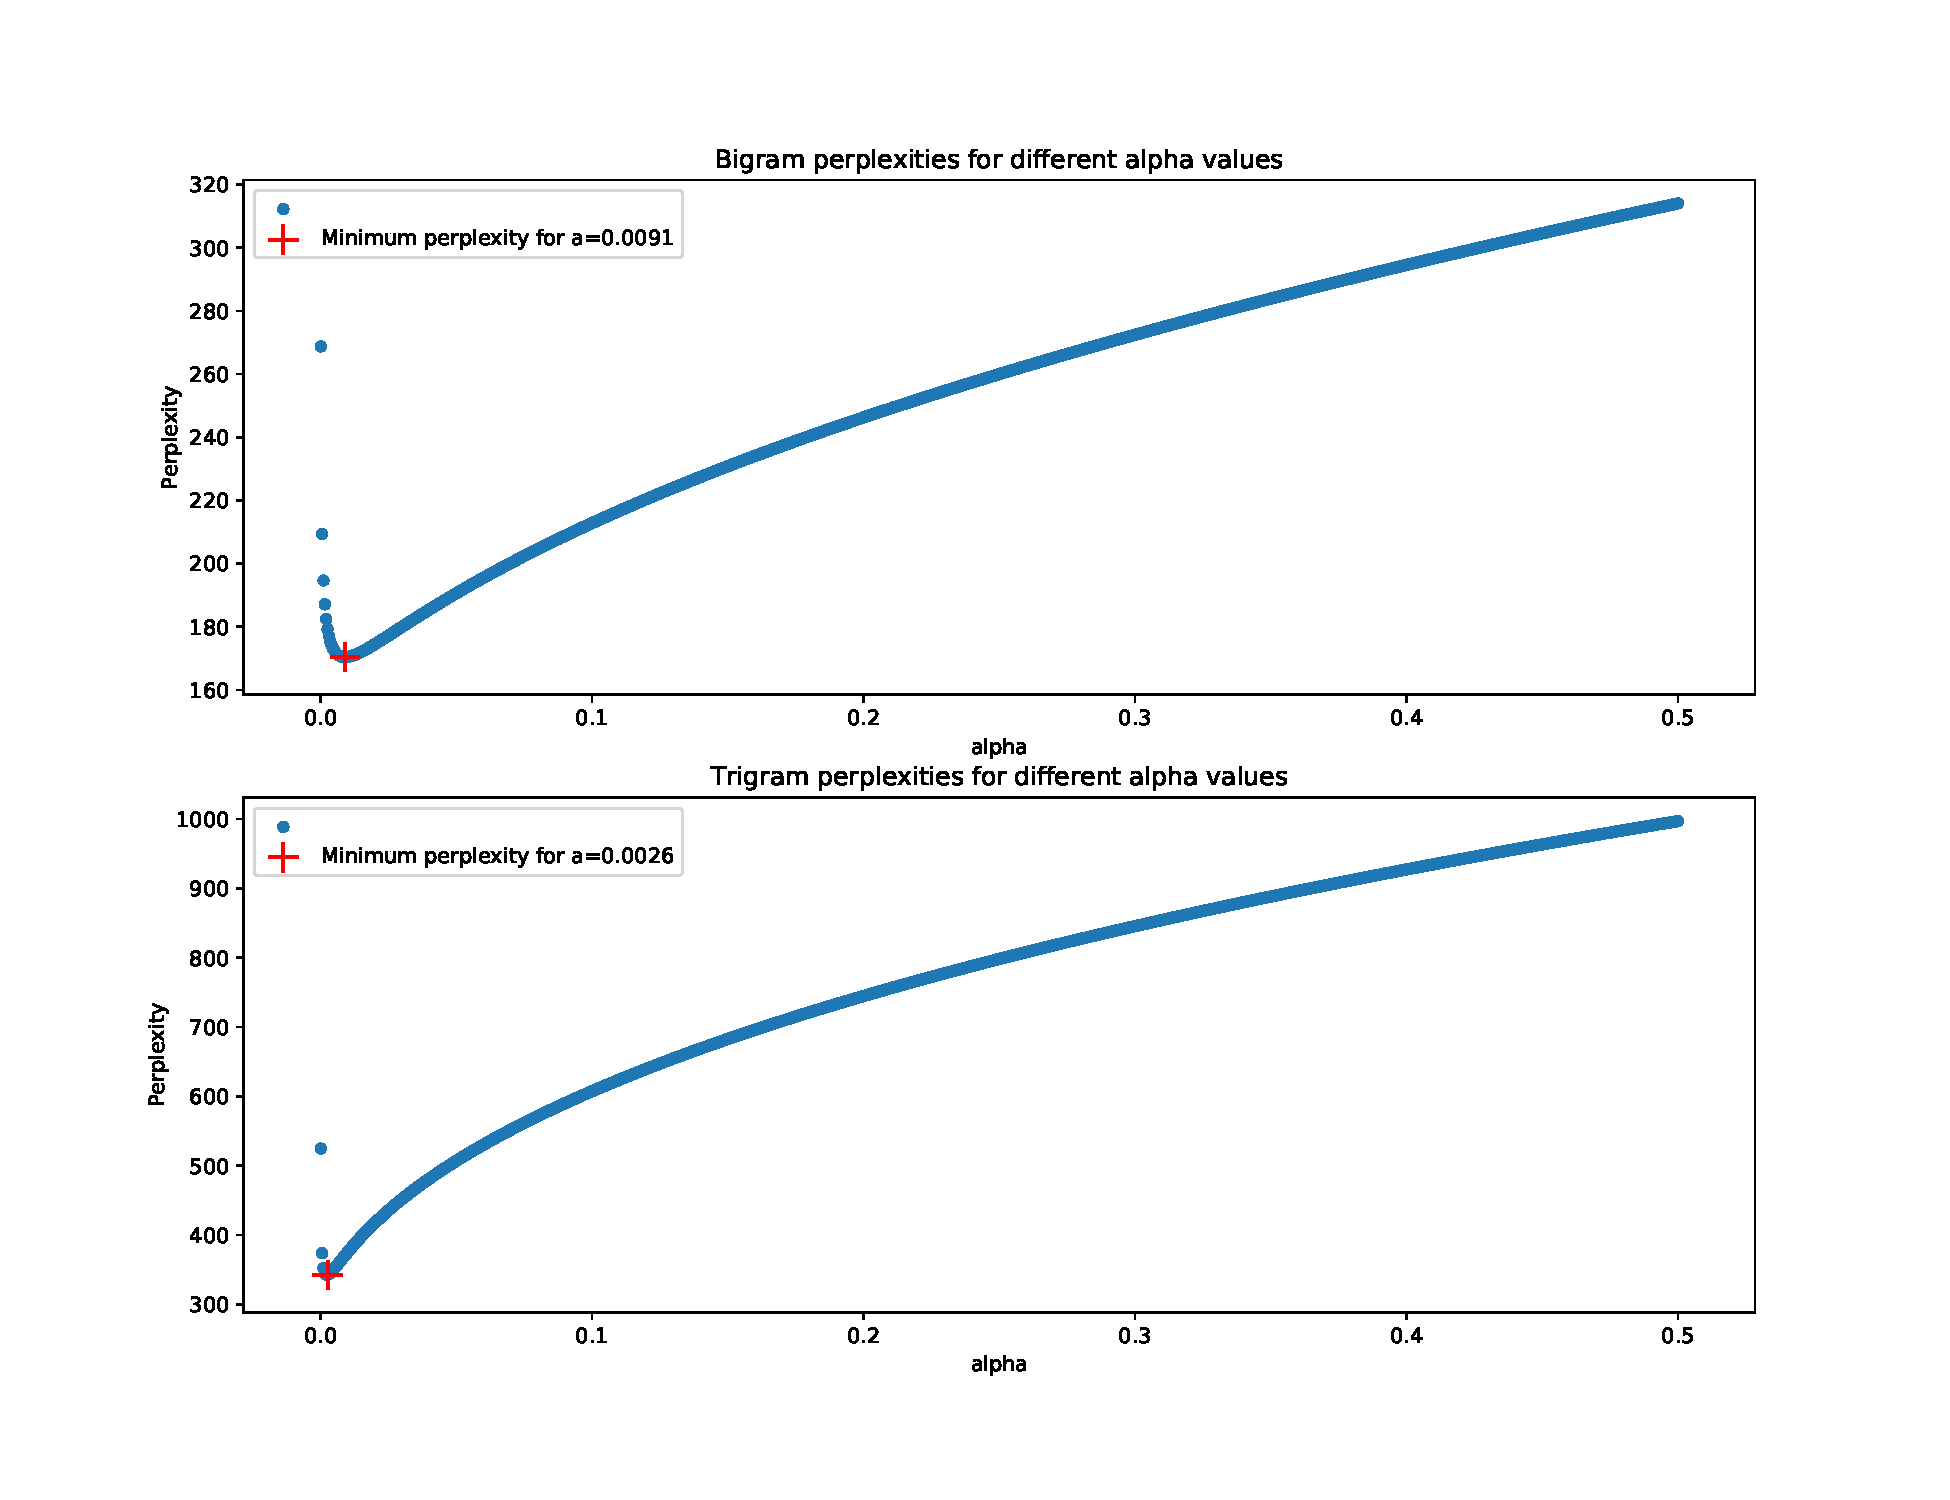
\includegraphics[width=\columnwidth]{Alpha_Tuning.pdf}
\end{figure}

\newpage

Using the values for the optimal alpha parameters ( \textit{$0.008$} for bigrams and \textit{$0.002$} for trigrams) and utilizing the method we created, for the calculation of cross-entropy and perplexity, we find and print the values of these two metrics. The same process is followed for both language models. From the results we obtained, we can see that both the values of perplexity and cross-entropy for the bi-gram language model are lower (e.g. better) than those of the tri-gram models.

\bigskip
\textbf{Bi-gram language model :}
\begin{verbatim}
Cross Entropy: 7.439
perplexity: 173.530
\end{verbatim}

\textbf{Tri-gram language model :}
\begin{verbatim}
Cross Entropy: 8.467
perplexity: 353.731
\end{verbatim}

\subsection*{Part iv} 
For the fourth and last part of this exercise, we have to combine our two models using linear interpolation and check if the combined model performs better in terms of cross-entropy and perplexity. We also have to tune the lamda hyper-parameter on a development subset of the corpus. 

We start, by creating a function (\textcolor{red}{int\_log\_prob}) which returns the sum probability from both models, given that we have provided a set of tokenized sentences, a value for the lamda parameter and both the values of alphas\footnote{we use the optimal alphas that we found earlier.} for each of the language models.


\begin{equation*}
P(w_3 | w_1, w_2) = \lambda P(w_3 | w_1, w_2) + (1-\lambda) P(w_3 |w_2), \quad \lambda \in [0,1]
\end{equation*}

\newpage
Next, in order to tune the lamda hyper-parameter, we found the perplexity for \textbf{1000} values for lamda and created the following graph.
\begin{figure}[!h]
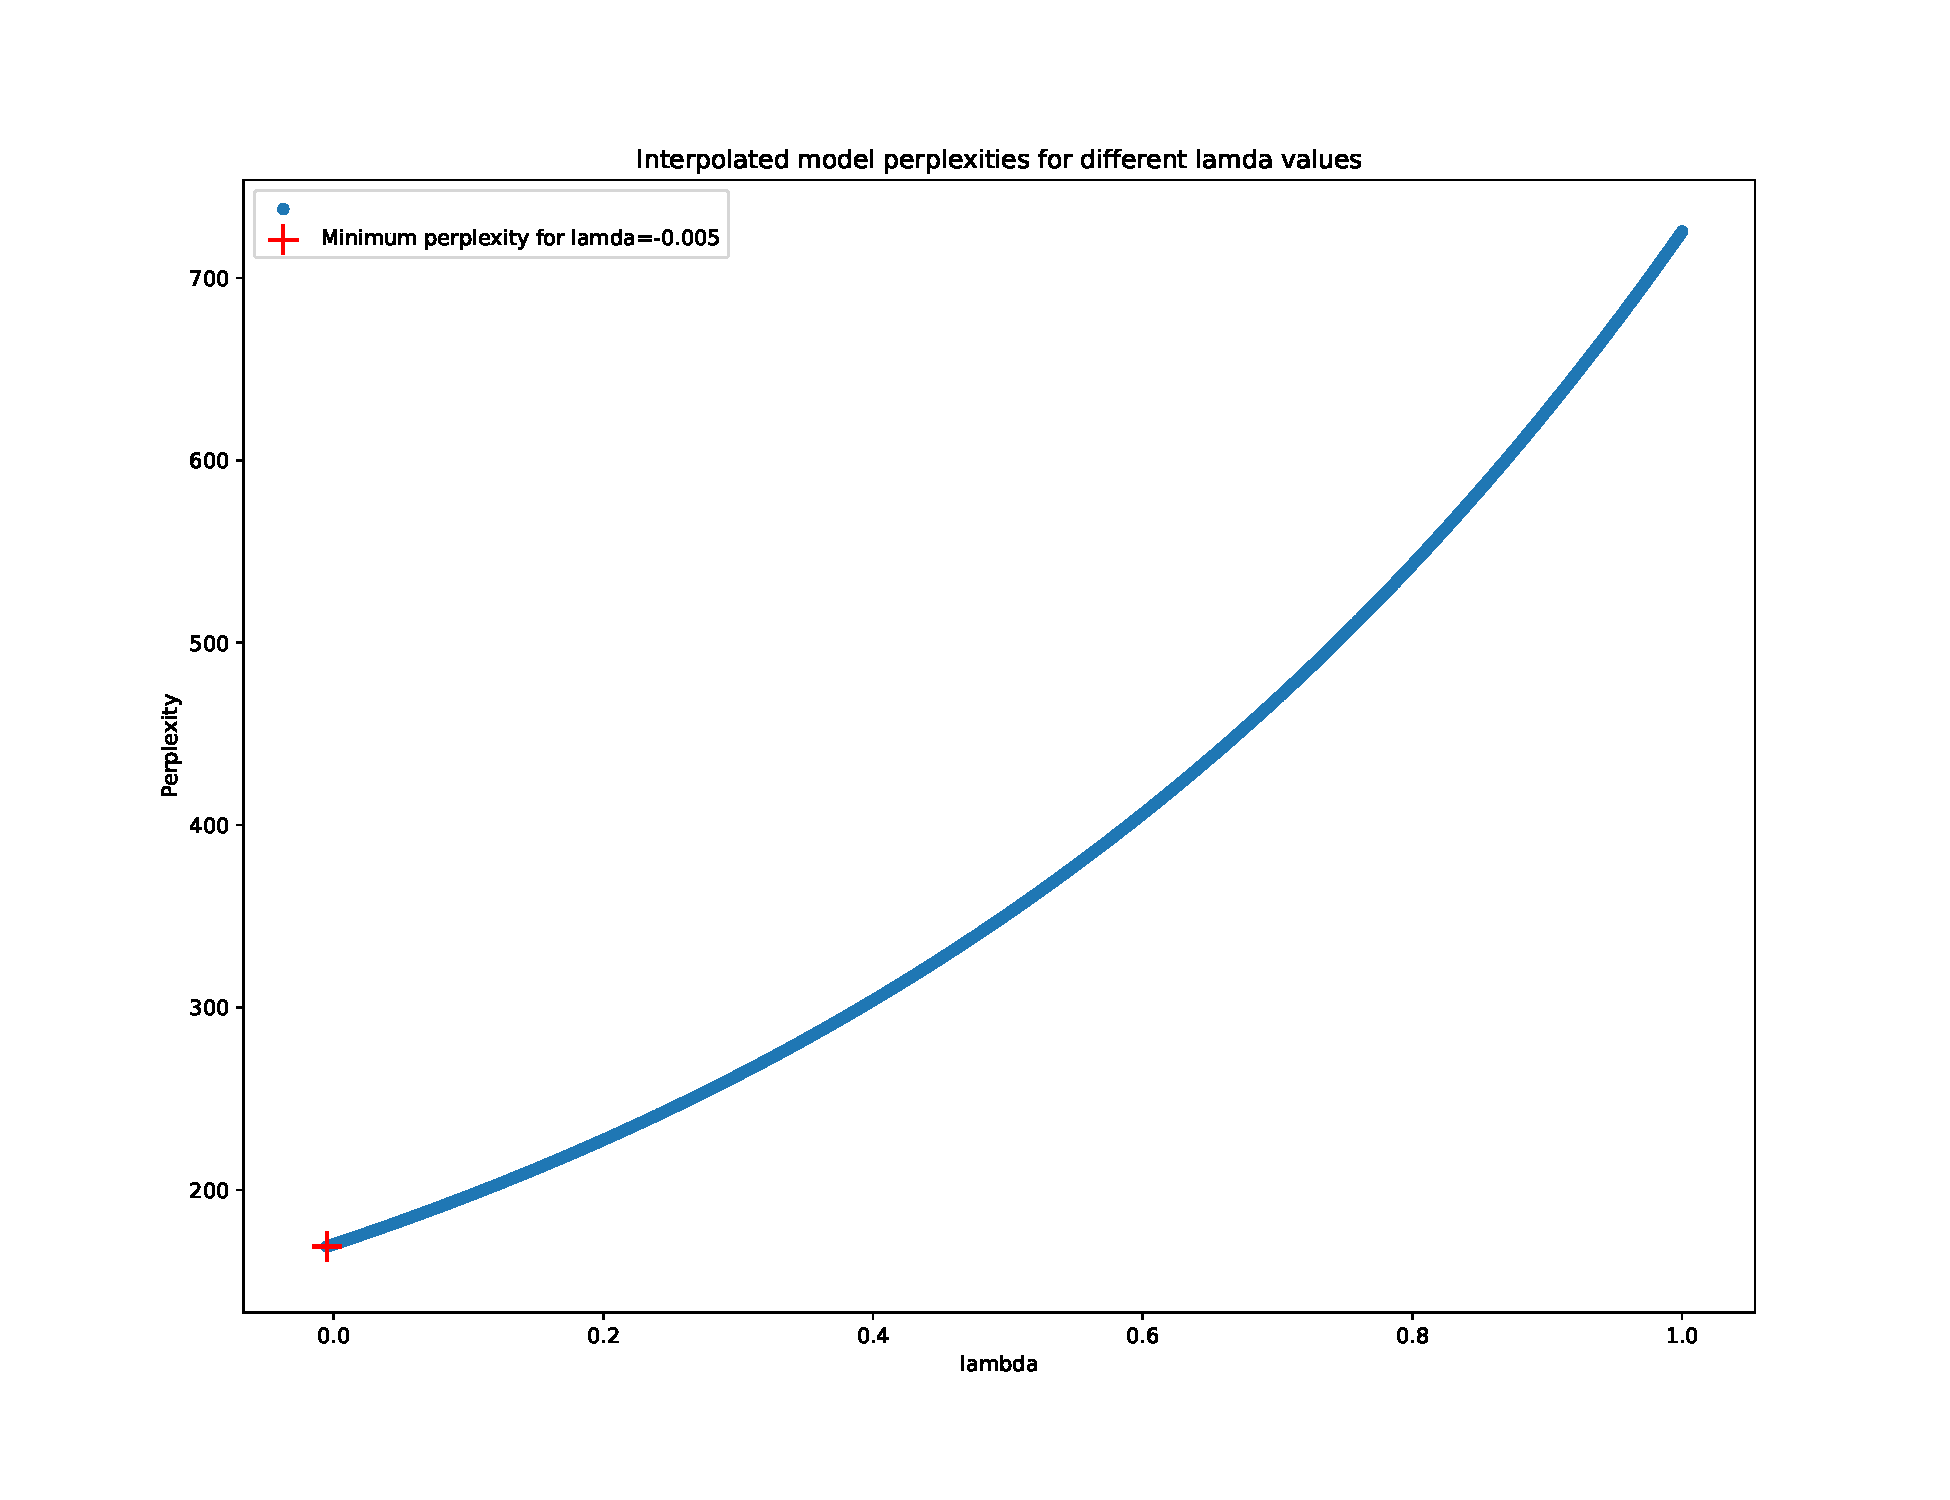
\includegraphics[width=\columnwidth]{Lambda_Tuning.pdf}
\end{figure}

The graph, shows that perplexity is always increasing in value and so, simply the best lamda value for us would be the lowest, which is 0.
\footnote{The model tends to be a bi-gram in order to reduce the language cross-entropy.} 
But, for the purpose of demonstrating the performance of an interpolated model, we arbitrarily choose $\lambda = 0.1$ ,thus

\bigskip
\textbf{Interpolated language model :}
\begin{verbatim}
Cross Entropy: 7.649
perplexity: 200.730
\end{verbatim}
%add kneser description


\newpage
\subsection*{Appendix A: Kneser-ney smoothing} 
We estimate the language cross entropy and perplexity of our models using Kneser-ney smoothing.
\footnote{https://github.com/smilli/kneser-ney/} 
We use the following formula:

\begin{align*}
P_{KN}(w_k | w_k-1) =  \begin{cases}  \frac{c(w_{k-1},w_k)-D}{c(w_{k-1})} & c(w_{k-1},w_k) > 0 \\ \alpha w_{k-1} P(w_k) & else \end{cases}
\end{align*}

where 
\begin{itemize}
\item $c(w_{k-1})$: unigram count
\item $c(w_{k-1},w_k)$: bigram count
\item $\alpha$: normalization constant  
\end{itemize}


From the results we obtained, we can see that both the values of perplexity and cross-entropy for the two language models are lower (e.g. better) than those of the part iii.

\bigskip
\textbf{Bi-gram language model :}
\begin{verbatim}
Cross Entropy: 3.439
perplexity: 10.85
\end{verbatim}

\textbf{Tri-gram language model :}
\begin{verbatim}
Cross Entropy: 3.687
perplexity: 12.88
\end{verbatim}

 
 




























\end{document}

